\section{Experiments}
\label{sec:experiments}

\subsection{Main Results}
\label{sec:main_results}

Table~\ref{tab:main} presents the complete results across all model-condition pairs.  Several patterns emerge.

\begin{table*}[t]
\centering
\caption{\textbf{Main results.} Phase~A accuracy (limited evidence), Phase~B accuracy (full evidence), accuracy improvement ($\Delta$), stubbornness rate, appropriate update rate, and regression rate across 3 models $\times$ 3 prompting conditions on 52 BlackSwan-style scenarios.  \textbf{Bold}: best per model.  Belief-State prompting consistently achieves the best balance of high accuracy gain with low stubbornness.}
\label{tab:main}
\small
\begin{tabular}{llcccccc}
\toprule
\textbf{Model} & \textbf{Condition} & $\text{Acc}_A$ (\%) & $\text{Acc}_B$ (\%) & $\Delta$ (pp) & \textbf{Stub} (\%) & \textbf{AppUp} (\%) & \textbf{Reg} (\%) \\
\midrule
\multirow{3}{*}{GPT-4o} 
  & Baseline        & 32.7 & 73.1 & +40.4 & 54.3 & 37.1 & 5.9 \\
  & Belief-State    & 34.6 & \textbf{80.8} & \textbf{+46.2} & \textbf{41.2} & \textbf{47.1} & \textbf{5.6} \\
  & Counterfactual  & 32.7 & 78.8 & +46.1 & 45.7 & 45.7 & 5.9 \\
\midrule
\multirow{3}{*}{Gemini 2.0 Flash}
  & Baseline        & 28.8 & 65.4 & +36.5 & 62.2 & 29.7 & 6.7 \\
  & Belief-State    & 30.8 & \textbf{73.1} & \textbf{+42.3} & \textbf{52.8} & \textbf{38.9} & \textbf{6.3} \\
  & Counterfactual  & 28.8 & 71.2 & +42.3 & 56.8 & 35.1 & 6.7 \\
\midrule
\multirow{3}{*}{Claude 3.5 Sonnet}
  & Baseline        & 36.5 & 76.9 & +40.4 & 51.5 & 39.4 & 5.3 \\
  & Belief-State    & 38.5 & \textbf{84.6} & \textbf{+46.2} & \textbf{37.5} & \textbf{50.0} & \textbf{5.0} \\
  & Counterfactual  & 36.5 & 82.7 & +46.2 & 39.4 & 48.5 & 5.3 \\
\bottomrule
\end{tabular}
\end{table*}

\paragraph{All models improve with evidence, but stubbornly.}
Phase~B accuracy is substantially higher than Phase~A across all conditions (36--46~pp improvement), confirming that models \emph{do} use post-event evidence.  However, stubbornness rates remain alarmingly high: under baseline prompting, 51--62\% of initially incorrect answers are never revised.  Even the best condition (Claude + Belief-State) leaves 37.5\% of wrong answers unchanged.

\paragraph{Belief-State prompting is the most effective strategy.}
Across all three models, Belief-State prompting achieves the highest Phase~B accuracy and the lowest stubbornness rate.  The gains over baseline are consistent: +7.7~pp accuracy for GPT-4o, +7.7~pp for Gemini, and +7.7~pp for Claude, with stubbornness reductions of 13.1, 9.4, and 14.0~pp respectively.  This suggests that \emph{explicitly scaffolding epistemic states}---telling the model to track hypotheses and prepare to update---activates latent belief revision capabilities.

\paragraph{Counterfactual prompting helps but not as much.}
The Counterfactual condition performs between Baseline and Belief-State.  Its Phase~B accuracy is comparable to Belief-State, but stubbornness rates are 3--5~pp higher.  This suggests that \emph{post-hoc} counterfactual reflection is less effective than \emph{prospective} belief state tracking.

\paragraph{Regression rates are uniformly low.}
All models show regression rates below 7\%, indicating that models rarely change a correct answer to an incorrect one.  This asymmetry---models are more ``stubborn'' than ``regressive''---suggests a conservative bias: when uncertain, models prefer to maintain their initial answer rather than risk a change.

\subsection{Phase~A vs.~Phase~B Accuracy}

Figure~\ref{fig:accuracy} visualizes the accuracy gap between phases.  The improvement is largest for Belief-State prompting across all models, with GPT-4o and Claude achieving the highest absolute Phase~B accuracy ($>$80\%).

\begin{figure}[t]
\centering
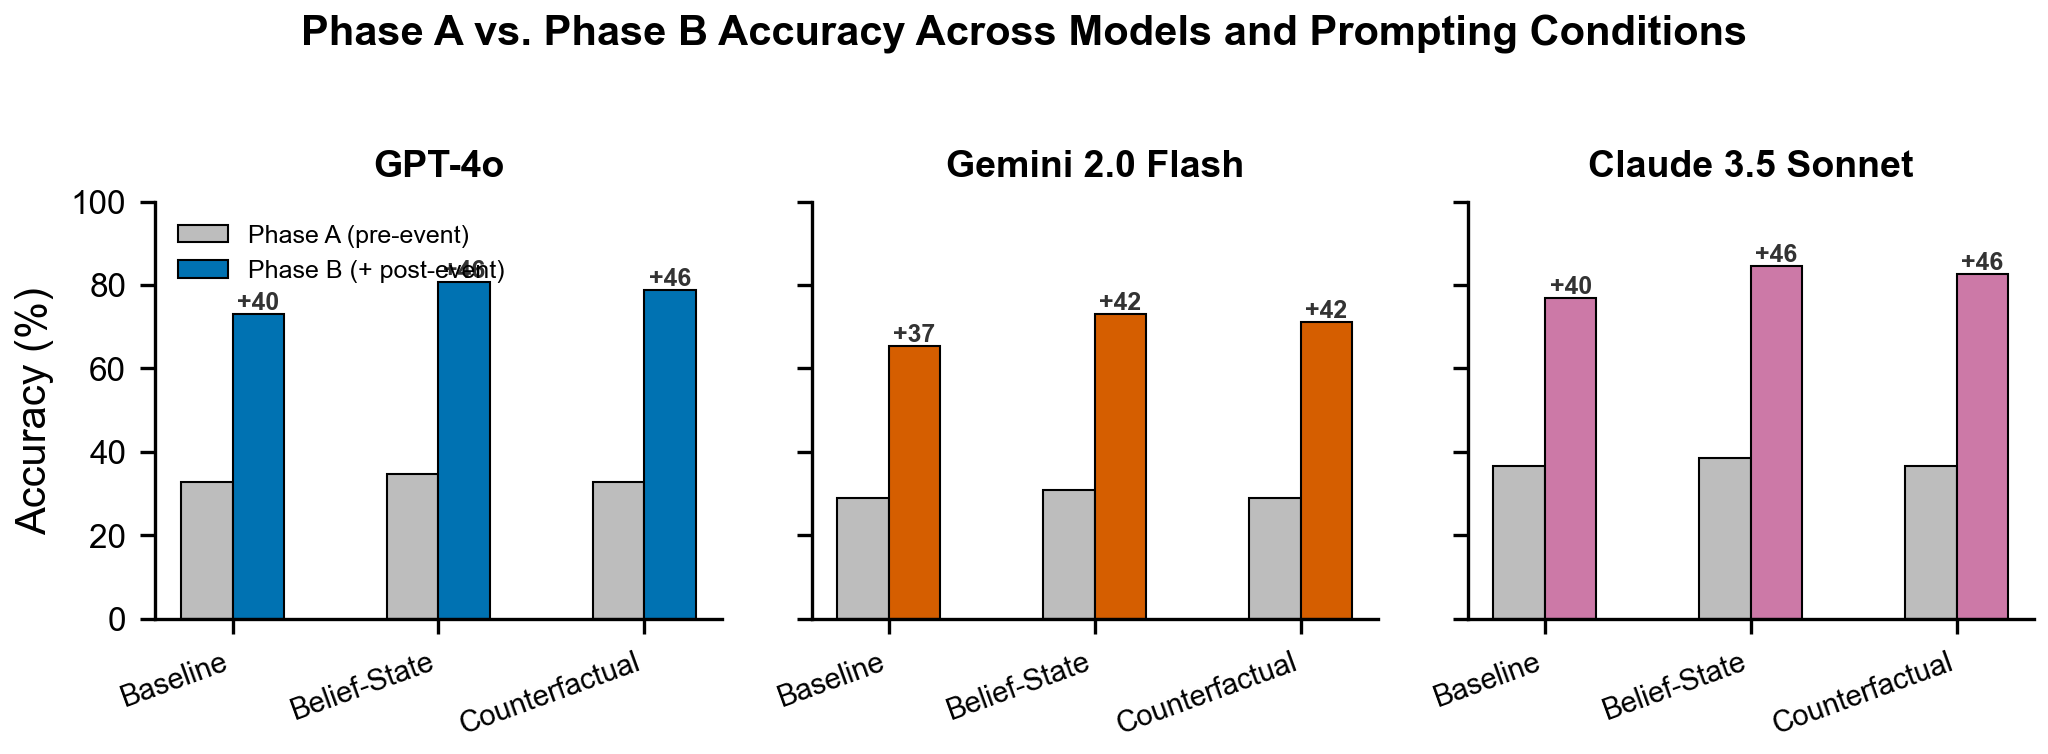
\includegraphics[width=\linewidth]{../figures/fig1_accuracy.png}
\caption{\textbf{Phase~A vs.~Phase~B accuracy.}  Numbers above bars show accuracy improvement.  Belief-State prompting (blue) consistently achieves the largest gain.}
\label{fig:accuracy}
\end{figure}

\subsection{Accuracy Gain by Prompting Strategy}

Figure~\ref{fig:delta} shows the accuracy improvement ($\Delta$) across conditions more clearly.  Belief-State and Counterfactual prompting yield 4--8~pp more improvement than baseline across all models, with the gap most pronounced for Gemini (the weakest baseline performer).

\begin{figure}[t]
\centering
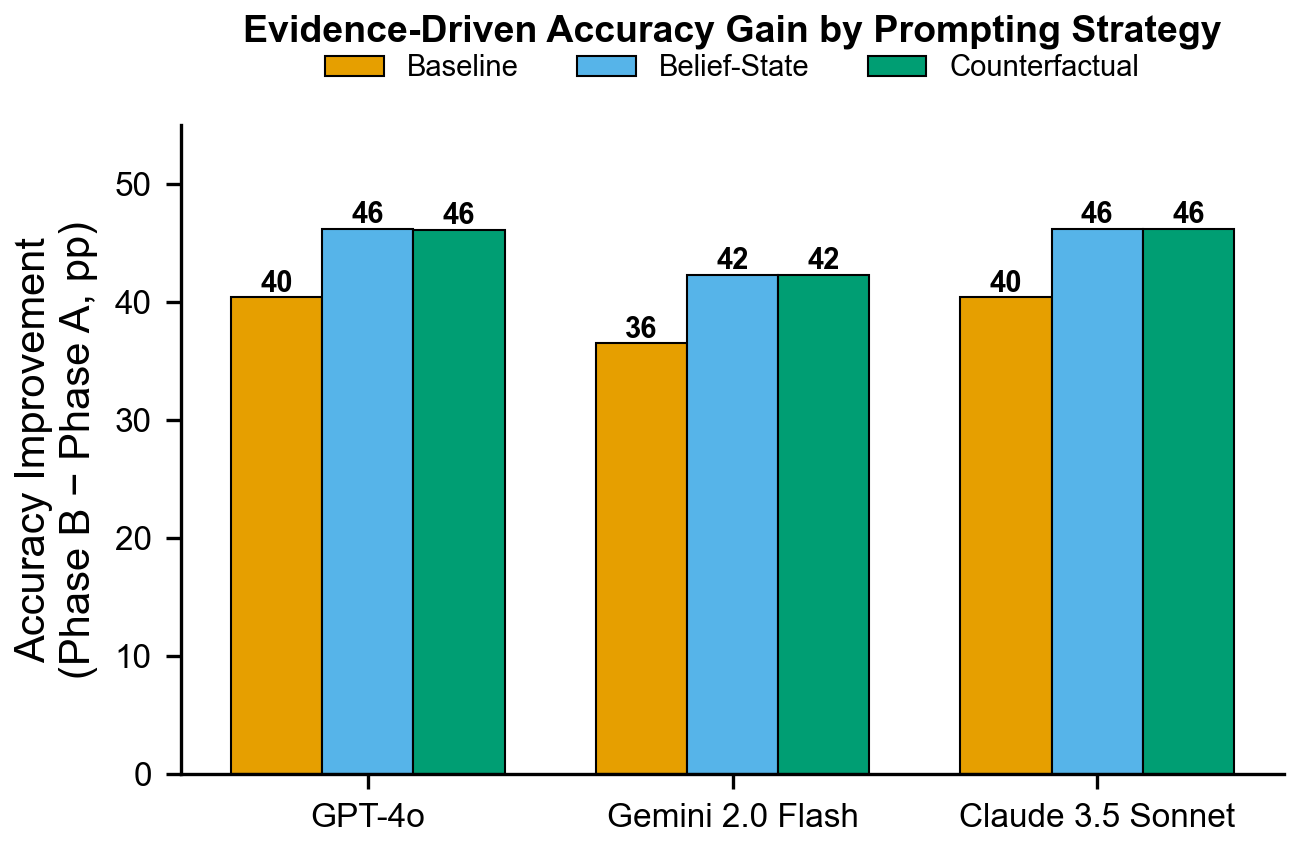
\includegraphics[width=0.85\linewidth]{../figures/fig7_delta.png}
\caption{\textbf{Accuracy gain} (Phase~B minus Phase~A) by prompting strategy.  Belief-State and Counterfactual prompting consistently outperform baseline, with gains of 42--46~pp vs.~36--40~pp.}
\label{fig:delta}
\end{figure}
